\documentclass[12pt]{article}

%%%%%%%%%%%%%%%%%
% the packages
\usepackage[utf8]{inputenc}
\usepackage[a4paper,margin=1in]{geometry}
\usepackage{graphicx,caption,subcaption}
\usepackage{color,hyperref}
\hypersetup{colorlinks=true,urlcolor=blue,citecolor=blue,linkcolor=blue}
\usepackage{enumitem}

\usepackage{multicol,longtable,multirow,booktabs,array}
\usepackage[authoryear]{natbib}
\bibliographystyle{plainnat}

\usepackage{mathaddons}

\newcommand{\sr}[1]{\textcolor{red}{#1}}


%%%%%%%%%%%%%%%%%%%%%%%%%
\title{Notes on High Dimension Probability}
\author{Subhrajyoty Roy}
\date{\today}


\begin{document}
\allowdisplaybreaks
\maketitle

\begin{abstract}
    This contains the lecture notes of the course on \textit{High Dimensional Probability} by Roman Vershynin. The course is available for free at online~\url{https://www.math.uci.edu/~rvershyn/teaching/hdp/hdp.html}.
\end{abstract}

\tableofcontents


\section{Introduction to High Dimensional Ideas}

\textbf{Big data} can come in one of two different ways.
\begin{enumerate}
	\item \# observations is big, this is usually easy, as classical statistical theory tells us how to deal with large number of samples. These are often better.
	\item \# dimensions is big. This is usually hard.
\end{enumerate}

Empirical observation: it is exponentially harder to deal with larger \# of dimensions rather than larger \# of observations. To illustrate this, let's consider an example problem.

\begin{example}
	Let's say we want to numerically compute the integral
	\begin{equation*} 
		\int_0^1 \cdots \int_0^1 f(x_1, \ldots, x_d) dx_1 \ldots dx_d
	\end{equation*}
	The usual way is to perform a numerical integration approach, based on Riemann sums. For $d = 1$, we can subdivide the interval $[0, 1]$ into grids of width (or resolution) $\epsilon$, so there are $1/\epsilon$-grids. Then, we have the Riemann sum as 
	\begin{equation*}
		\int_{[0, 1]} f(x)dx \approx \dfrac{1}{n}\sum_{i=1}^n f(x_i), \ n = (1/\epsilon).
	\end{equation*}
	\noindent Note that, this will ensure that the bias is of order $O(\epsilon)$, assuming $f$ is bounded. To see this,
    \begin{align*}
        \left\vert \int_{[0, 1]} f(x)dx - \dfrac{1}{n}\sum_{i=1}^n f(x_i) \right\vert
        & \leq \dfrac{1}{n}\sum_{i=1}^{n} \left\vert \int_{[(i-1)/n, i/n]} f(x)dx - f(x_i) \right\vert\\
        & = \dfrac{1}{n}\sum_{i=1}^{n} \left\vert f(t_i) - f(x_i) \right\vert\\
        & = O(1/n) = O(\epsilon)
    \end{align*}
    \noindent where $t_i$ is a tag obtained by using Integral Mean Value Theorem on $f$, for the interval $[(i-1)/n, i/n]$. 

    In general, for $d$-dimensional hypercube $[0, 1]^d$, we require $n = O(1/\epsilon^d)$ many points to achieve an error bound of $O(\epsilon)$.
\end{example}

Therefore, we need the number of points to be exponential in dimension to achieve the same level of accuracy. This is also called \textbf{the curse of dimensionality}.

However, there is a better way to solve this problem, by using Monte Carlo method, which uses probabily to achieve good result for this. Instead of choosing the points on the grid, choose uniformly at random. Pick $N$ points:

\begin{equation*}
    S_N = \dfrac{1}{N}\sum_{i=1}^N f(x_i), \ x_i \sim \text{Uniform}([0, 1]^d)
\end{equation*} 

Note that, $\E(S_N) = \E(f(X)) = \int_{[0, 1]^d} f(x)dx$. The average $L^2$ error is given by
\begin{align*}
    \E\left[\left(\frac{1}{N} \sum_{i=1}^N f(x_i) - \int_{[0,1]^d} f(x) dx\right)^2 \right] 
    & = \var\left( \frac{1}{N} \sum_{i=1}^N f(x_i) \right)\\
    & = \dfrac{\var(f(X))}{N} \leq C/N
\end{align*}
\noindent since $f(x)$ is bounded. Therefore, the RMSE = $O(\frac{1}{\sqrt{N}})$, independent of the dimension $d$. 

\begin{note}
    Thinking in terms of probability might help to overcome in high-dimensional inference problems.
\end{note}


\subsection{Convexity}

Usually in high-dimensional (HD) problems, convexity helps a lot.

\begin{definitionbox}
    A set $T \subset \R^n$ is convex if $\forall x,y \in T$, the segment $[x,y] \in T$.
\end{definitionbox}

Let us consider a few examples as follows:

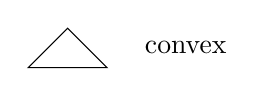
\begin{tikzpicture}[scale=0.5]
\draw (0,0) -- (1,1) -- (2,0) -- cycle;
\node at (4,0.5) {convex};
\end{tikzpicture}


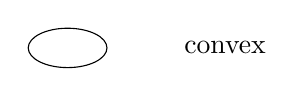
\begin{tikzpicture}[scale=0.5]
\draw (3,0) ellipse (1cm and 0.5cm);
\node at (7, 0) {convex};
\end{tikzpicture}


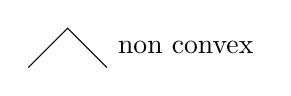
\begin{tikzpicture}[scale=0.5]
\draw (6,0) -- (7,1) -- (8,0);
\node at (10,0.5) {non convex};
\end{tikzpicture}


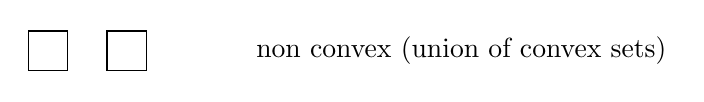
\begin{tikzpicture}[scale=0.5]
\draw (9,0) rectangle (10,1);
\draw (11,0) rectangle (12,1);
\node at (20,0.5) {non convex (union of convex sets)};
\end{tikzpicture}

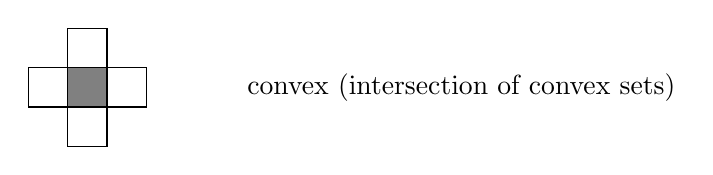
\begin{tikzpicture}[scale=0.5]
\draw (5,0) rectangle (8,1);
\draw (6,-1) rectangle (7,2);
\draw[fill = gray] (6,0) rectangle (7,1);
\node at (16,0.5) {convex (intersection of convex sets)};
\end{tikzpicture}

This means union of convex sets may not be convex, but intersection of convex sets is convex. Thus, starting with a set $T$, we can consider the intersection of all such convex sets that are superset of $T$.

\begin{definitionbox}
    The convex hull $\text{conv}(T)$ of a set $T \subset \R^n$ is the smallest convex set that contains $T$.
\end{definitionbox}

\begin{theorembox}
    $\forall z \in \text{conv}(T)$, we have a decomposition, $z = \sum_{i=1}^m \lambda_i z_i$, where, $\lambda_i \geq 0$, $\sum_{i=1}^m \lambda_i = 1$, and each $z_i \in T$. Note that, the above combination or representation may not be unique or parsimonious.
\end{theorembox}

\begin{theorembox}[Caratheodory Theorem]
    $\forall z \in \text{conv}(T)$, $\exists$ a representation (convex combination) of $\leq (n+1)$ points in $T$, where, $T \subset \R^n$.
\end{theorembox}

Note that, the choice of basis in the representation obtained by Caratheodory Theorem may depend on the choice of $z$. Also, the number $(n+1)$ is unimprovable, there is a dimension dependence here. However, it turns out if we allow to get $z$ back only approximately, we can use a similar trick like the Monte Carlo method of get a better representation, that may be dimension-independent.

\begin{theorembox}[Approximate Caratheodory Theorem]
    Let $T \subset \R^n$, and $\text{diam}(T) \leq 1$ (otherwise we can rescale). Then, $\forall z \in \text{conv}(T)$, $\forall k \in \N$, $\exists z_1, z_2, \ldots, z_k \in T$ (these points may be same) such that
    \begin{equation*}
        \left\Vert z - \frac{1}{k} \sum_{i=1}^k z_i\right\Vert_2 \leq \frac{1}{\sqrt{2k}}
    \end{equation*}
    This means, if we want error to be less than equal to $\epsilon$, the choose, $k = \frac{1}{2\epsilon^2}$ (which is dimension free).
\end{theorembox}

\begin{proof}
    
\end{proof}



\textbf{Proof (empirical method f./ Maurey):}

Fix any $z \in \text{conv}(T)$, by Caratheor Fact, we have,
$z = \sum_{i=1}^m \lambda_i z_i$, $\lambda_i \geq 0$, $\sum_{i=1}^m \lambda_i = 1$, $z_i \in T$.

Consider a r.v. $Z$ that takes value $z_i$, with prob $\lambda_i$.

Then, $z = \sum_{i=1}^m \lambda_i z_i = \mathbb{E}Z$. Consider iid copies of $Z$, as, $X_1, X_2, \ldots, X_k \equiv Z$

So, Error $=\mathbb{E}\left(\left\|z - \frac{1}{k} \sum_{i=1}^k X_i\right\|_2^2\right) = \mathbb{E}\left\|\frac{1}{k} \sum_{i=1}^k (X_i - z)\right\|_2^2$
$= \frac{1}{k^2} \sum_{i=1}^k \mathbb{E}\left\|X_i - \mathbb{E}X_i\right\|_2^2$, since, $z = \mathbb{E}Z = \mathbb{E}X_i$, $\forall i$
$= \frac{1}{k} \mathbb{E}\left\|Z - \mathbb{E}Z\right\|_2^2$ (since $X_i \equiv Z$)
$= \frac{1}{2k} \mathbb{E}\left\|Z - Z'\right\|_2^2$ (where, $Z'$ is an indep copy of $Z$)
$\leq \frac{1}{2k}$, as, $\left\|Z-Z'\right\|_2^2 \leq \text{diam}(T) \leq 1$.

$\Rightarrow$ So since, the expectation $\leq \frac{1}{2k} \Rightarrow \exists$ a realization of $X_i$'s s.t. error $\leq \frac{1}{2k}$

$\Rightarrow \left\|z - \frac{1}{k} \sum_{i=1}^k z_i\right\|_2^2 \leq \frac{1}{2k}$, where, $z_i$'s are the realizations of $X_i$
$\uparrow$
$\in T$.


\section*{Lec 3}

\textbf{Applications of ACT:}
\begin{itemize}
    \item Portfolio building - ingredients = stocks
    
    linear/convex comb of them $\rightarrow$ mutual funds
    
    \textbf{Problem:} Create a new MF with a given combination of stocks by mixing available MFs. (Fund of funds)
    
    \textbf{Solution:} ACT provides a fast randomized solution (approximately)
    
    \item Covering Numbers:
    
    \textbf{Def:} The covering \# of a set $T \subset \mathbb{R}^n$ at scale $\epsilon > 0$ is the smallest \# of Euclidean balls of radius $\epsilon$ needed to cover $T$. Denote by $N(T,\epsilon)$
    
    example:
    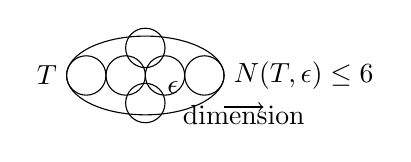
\begin{tikzpicture}[scale=0.5]
    \draw (0,0) ellipse (2cm and 1cm);
    \draw (0.5,0) circle (0.5cm);
    \draw (-0.5,0) circle (0.5cm);
    \draw (1.5,0) circle (0.5cm);
    \draw (-1.5,0) circle (0.5cm);
    \draw (0,0.7) circle (0.5cm);
    \draw (0,-0.7) circle (0.5cm);
    \node at (-2.5,0) {$T$};
    \node[right] at (2,0) {$N(T,\epsilon) \leq 6$};
    \node at (2.5,-1) {dimension};
    \draw[->] (2,-0.8) -- (3,-0.8);
    \node at (0.7,-0.3) {$\epsilon$};
    \end{tikzpicture}
    
    \textbf{Fact 1:} $B$ = unit euclidean ball, we have $N(B, \frac{1}{2}) \geq 2^{0.2d}$ \hspace{2cm} (exponentially large)
    
    \textbf{Proof:} Assume $B$ can be covered by $N$ copies of $(\frac{1}{2}B)$ ball.
    
    $Vol(B) \leq N \cdot Vol(\frac{1}{2}B)$ \hspace{2cm} (RHS might have some overlap)
    
    $\Rightarrow Vol(B) \leq N \cdot (\frac{1}{2})^d Vol(B) \Rightarrow N \geq 2^d$.
    
    \textbf{Fact 2:} Let $P$ be a polytope in $\mathbb{R}^d$ with $m$ vertices, $diam(P) \leq 1$. Then,
    
    $N(P, \epsilon) \leq m^{\frac{1}{2\epsilon^2}}$ \hspace{1cm} (polynomial in $m$, nontrivial
    \begin{tabular}{l}
    since, in $\mathbb{R}^3$, $\exists$ a polytope with $m = O(d)$ \\
    vertices, \\
    we have, RHS = polynomial in d)
    \end{tabular}
    
    dimension free
    
    \textbf{Proof:} Consider, $P$ is nonconvex, then $conv(P)$ is a polytop with $\leq m$ vertices.
    
    So, w.l.o.g. assume $P$ is convex.
    
    Let $T = \{vertices\text{ of }P\}$, clearly, $P \subset conv(T)$.
    
    ACT $\Rightarrow$ $\forall z \in P$, is within distance $\frac{1}{\sqrt{2k}}$ from some point in the
    
    set $\mathcal{N} := \{\frac{1}{k} \sum_{i=1}^k z_i : z_i \in T\}$
    
    $\Rightarrow \forall x \in P$, is covered by a ball of radius $\frac{1}{\sqrt{2k}}$ and center $\in \mathcal{N}$.
    
    $\Rightarrow N(P, \frac{1}{\sqrt{2k}}) \leq |\mathcal{N}| \leq m^k$ \hspace{1cm} ($m$ vertices, each has $k$ elements)
    
    $\Rightarrow N(P, \epsilon) \leq m^{\frac{1}{2\epsilon^2}}$
\end{itemize}

Usually it helps by considering the intuition that, small covering \# $\Rightarrow$ small volume
$\Rightarrow$ easier to apply union type bounds

\section*{Lec 4}

Since covering \# of polytope is small, we expect volume of polytope is small.

\textbf{Thm (Carl-Pajor '88):} Let $B$ = euclidean ball, $P \subset B$ any polytope with $m$ vertices in $\mathbb{R}^n$

Then, $\frac{Vol(P)}{Vol(B)} \leq \left(4\sqrt{\frac{\log m}{n}}\right)^n$ \hspace{1cm} (unless $m$ is exponential in $n$, the RHS is exponentially small)

\textbf{Proof:} We consider $\epsilon B$-balls and cover $P$ with these.

By def'n of covering \#, $Vol(P) \leq N(P,\epsilon) \cdot Vol(\epsilon B)$
$\Rightarrow Vol(P) \leq N(P,\epsilon) \cdot \epsilon^n Vol(B)$
$\Rightarrow \frac{Vol(P)}{Vol(B)} \leq \epsilon^n \cdot m^{\frac{1}{2\epsilon^2}}$ \hspace{1cm} ($m^{\frac{1}{\epsilon^2}} \approx diam(P) \leq diam(B) \leq 2$)

holds for $\forall \epsilon > 0$

$\Rightarrow \frac{Vol(P)}{Vol(B)} \leq \inf_{\epsilon > 0} \epsilon^n \cdot m^{\frac{1}{2\epsilon^2}}$

Let $\ell(\epsilon) = \epsilon^n m^{\frac{1}{2\epsilon^2}} \Rightarrow \log \ell(\epsilon) = n \log \epsilon + \frac{1}{2\epsilon^2} \log m$
$\Rightarrow \frac{\partial \log l}{\partial \epsilon} = 0 = \frac{n}{\epsilon} - \frac{1}{\epsilon^3} \log m \Rightarrow \epsilon = \sqrt{\frac{4 \log m}{n}}$

$\Rightarrow \inf_{\epsilon > 0} \ell(\epsilon) = \exp\left[n \cdot \log \left(\sqrt{\frac{4 \log m}{n}}\right) + \frac{2 \log m}{4 \log m} \cdot n\right]$
$= \exp\left[\frac{n}{2} \log\left(\left(\sqrt{\frac{4 \log m}{n}}\right)^2 \cdot e^{\frac{n}{2}}\right)\right] = \left(\sqrt{\frac{4e \log m}{n}}\right)^n$
$\leq \left(4\sqrt{\frac{\log m}{n}}\right)^n$, as req'd

\textbf{Remarks:}
\begin{itemize}
    \item [CPT] proved a slightly better result, with $\log(m/n) \rightarrow$ optimal.
    \item The optimal bound is attained at a random polytope. (Dafnis et al., 2003, 2009)
    \item Let $S = 4\sqrt{\frac{\log m}{n}}$, note that, $Vol(SB) = S^n \cdot Vol(B)$
    $\Rightarrow \frac{Vol(SB)}{Vol(B)} = S^n \geq \frac{Vol(P)}{Vol(B)}$
    $\Rightarrow Vol(SB) \geq Vol(P)$
\end{itemize}

This means, the intuitive low-dimensional picture is wrong.

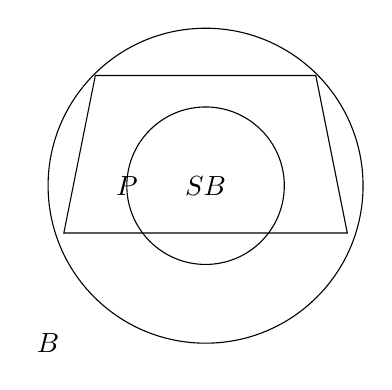
\begin{tikzpicture}
\draw (0,0) circle (2cm);
\draw (0,0) circle (1cm);
\draw (-1.8,-0.6) -- (-1.4,1.4) -- (1.4,1.4) -- (1.8,-0.6) -- cycle;
\node at (-1,0) {$P$};
\node at (0,0) {$SB$};
\node at (-2,-2) {$B$};
\end{tikzpicture}

\hspace{2cm} "V. Milman's" hyperbolic correction

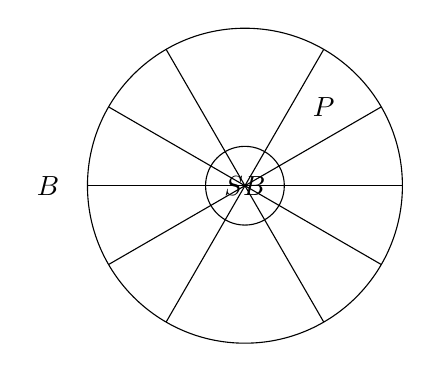
\begin{tikzpicture}
\draw (0,0) circle (2cm);
\draw (0,0) circle (0.5cm);
\draw (0,0) -- (2,0);
\draw (0,0) -- (1.73,1);
\draw (0,0) -- (1,1.73);
\draw (0,0) -- (-1,1.73);
\draw (0,0) -- (-1.73,1);
\draw (0,0) -- (-2,0);
\draw (0,0) -- (-1.73,-1);
\draw (0,0) -- (-1,-1.73);
\draw (0,0) -- (1,-1.73);
\draw (0,0) -- (1.73,-1);
\node at (1,1) {$P$};
\node at (0,0) {$SB$};
\node at (-2.5,0) {$B$};
\end{tikzpicture}

often called the "core" \hspace{2cm} $P$ - is convex (not look like so)

\textbf{Concentration Inequalities:}

$X \approx \mathbb{E}X$ with high probability (exponentially close to 1).

\textbf{Example (Normal dist):} 

\[ X \sim N(\mu, \sigma^2) \quad \text{and} \quad \mathbb{P}(|X - \mu| > t\sigma) \approx 0.9987 \]

\textbf{Prop (Gaussian tails):}

\[ g \sim N(0,1) \quad \text{and} \quad \mathbb{P}(g > t) \leq \frac{1}{\sqrt{2\pi}} \int_{t}^{\infty} e^{-x^2/2} \, dx \approx \frac{1}{\sqrt{2\pi}} \frac{e^{-t^2/2}}{t} \quad \text{(decay exp fast in $t$)} \]

\textbf{Proof:}

\[ \mathbb{P}(g > t) = \int_{t}^{\infty} \frac{1}{\sqrt{2\pi}} e^{-x^2/2} \, dx = \int_{0}^{\infty} \frac{1}{\sqrt{2\pi}} e^{-(t+y)^2/2} \, dy \]

Using \( e^{-(t+y)^2/2} = e^{-t^2/2} \cdot e^{-ty} \cdot e^{-y^2/2} \):

\[ \leq \frac{1}{\sqrt{2\pi}} e^{-t^2/2} \int_{0}^{\infty} e^{-ty} e^{-y^2/2} \, dy \leq \frac{1}{\sqrt{2\pi}} e^{-t^2/2} \]

By symmetry, we then have:

\[ \mathbb{P}(|X - \mu| > t\sigma) = \mathbb{P}(|g| > t) \leq \frac{2}{\sqrt{2\pi}} \frac{e^{-t^2/2}}{t} \]

\[ X \sim N(\mu, \sigma^2) \]

\textbf{Turns out that the CLT tells:}

\[ \sqrt{n} \left(\frac{\bar{X} - \mu}{\sigma}\right) \to Z \sim N(0,1) \]

but the error here is of order \( \frac{1}{\sqrt{n}} \) (Berry-Esseen bound).

So, the tail of \( \sqrt{n} \left(\frac{\bar{X} - \mu}{\sigma}\right) \) does not go exponential like Gaussian. 

Concentration inequalities bridge that gap by controlling the tail bounds.

\textbf{For general distributions, we have:}

- \textbf{Markov inequality:} (For any nonnegative \( X \))

\[ \mathbb{P}(X \geq t) \leq \frac{\mathbb{E}X}{t}, \quad \text{where } t > 0 \]

- \textbf{Chebyshev's inequality:} \( X \) r.v. with mean \( \mu \), variance \( \sigma^2 \)

\[ \mathbb{P}(|X - \mu| \geq t) \leq \frac{\sigma^2}{t^2}, \quad \text{where } t > 0 \]

\textbf{Example:} Toss a fair coin \( N \) times. What is \( \mathbb{P}(\text{at least } \frac{3N}{4} \text{ heads}) \)?

Based on Chebyshev's inequality, \( S_N = \# \text{ of heads } \sim \text{Binomial}(N, \frac{1}{2}) \):

\[ \mathbb{E}S_N = \frac{N}{2}, \quad \text{var}(S_N) = \frac{N}{4} \]

\[ \mathbb{P}\left(S_N \geq \frac{3N}{4}\right) = \frac{1}{2} \mathbb{P}\left(|S_N - \frac{N}{2}| \geq \frac{N}{4}\right) \leq \frac{N/4}{(N/4)^2} = \frac{4}{N} = O\left(\frac{1}{N}\right) \]

\textbf{Based on CLT:}

\[ \frac{S_N - \mathbb{E}S_N}{\sqrt{\text{var}(S_N)}} \to Z \sim N(0,1) \quad \text{by CLT} \]

\[ \mathbb{P}\left(S_N \geq \frac{3N}{4}\right) = \mathbb{P}\left(\frac{S_N - \frac{N}{2}}{\sqrt{N/4}} \geq \frac{\sqrt{N/4}}{2}\right) \leq e^{-N/8} \]

But by Berry-Esseen bound, this error is \( O\left(\frac{1}{\sqrt{N}}\right) \).


\textbf{Theorem: (Berry-Esseen)}

Let \( X_i \) be i.i.d. r.v.s with mean 0, variance 1. Then

\[
\left| \mathbb{P}\left(\frac{1}{\sqrt{n}}\sum_{i=1}^{n} X_i \geq t\right) - \mathbb{P}(Z \geq t) \right| \leq \frac{\mathbb{E}|X_1|^3}{\sqrt{n}} = O\left(\frac{1}{\sqrt{n}}\right)
\]

This is an optimal order \( \frac{1}{\sqrt{n}} + e^{-Nt^2/2} \). This is worse than Chebyshev's.

So, the CLT method yields a bound of \( O\left(\frac{1}{\sqrt{n}} + e^{-Nt^2/2}\right) \). So the idea is to sidestep CLT and directly aim at controlling the tails.

\textbf{Theorem: (Hoeffding's Inequality)}

Let \( X_1, X_2, \dots, X_n \) be symmetric Bernoulli r.v.: \( \mathbb{P}(X_i = \pm 1) = \frac{1}{2} \). Then

\[
\mathbb{P}\left(\frac{1}{\sqrt{n}} \sum_{i=1}^{n} X_i \geq t\right) \leq e^{-t^2/2}, \quad \forall t \geq 0 \quad \text{(Gaussian tail)}
\]

\textbf{Proof (MGF method):}

Let \( \lambda > 0 \) be a parameter.

\[
\mathbb{P}\left(\frac{1}{\sqrt{n}} \sum_{i=1}^{n} X_i \geq t\right) = \mathbb{P}\left(e^{\lambda \sum_{i=1}^{n} X_i} \geq e^{\lambda t \sqrt{n}}\right) \leq e^{-\lambda t \sqrt{n}} \mathbb{E}\left(e^{\lambda \sum_{i=1}^{n} X_i}\right)
\]

(By Markov)

\[
= e^{-\lambda t \sqrt{n}} \prod_{i=1}^{n} \mathbb{E}\left(e^{\lambda X_i}\right) \quad \text{(since \(X_i\) are i.i.d)}
\]

\[
\leq e^{-\lambda t \sqrt{n}} \left(\frac{e^{\lambda} + e^{-\lambda}}{2}\right)^n \quad \text{[Note, cosh(\(\lambda\)) = \(\frac{e^{\lambda} + e^{-\lambda}}{2}\)]}
\]

\[
\leq e^{-\lambda t \sqrt{n}} e^{n\lambda^2/2} = \exp\left(-\lambda t \sqrt{n} + \frac{n \lambda^2}{2}\right)
\]

\[ 
\text{Minimize over } \lambda > 0.
\]

\textbf{Application (Mean Estimation):}

Let \( X_1, X_2, \dots, X_n \) be \( \text{i.i.d. } N(\mu, \sigma^2) \).

\textbf{Classical estimator:}

\[
\hat{\mu} = \frac{1}{N} \sum_{i=1}^{n} X_i, \quad \mathbb{E} \hat{\mu} = \mu \quad \text{(unbiased)}
\]

\[
\mathbb{E}\left(\hat{\mu} - \mu\right)^2 = \text{Var}(\hat{\mu}) = \frac{\sigma^2}{N} \Rightarrow \text{RMSE} = \frac{\sigma}{\sqrt{N}}
\]

\textbf{Confidence interval:}

\[
\mathbb{P}\left(|\hat{\mu} - \mu| \geq t \frac{\sigma}{\sqrt{N}}\right) \leq \frac{\sigma^2/N}{(t \sigma/\sqrt{N})^2} = \frac{1}{t^2} \quad \text{=> not very sharp bound.}
\]

Can we get sharper exponentially close to 1 confidence for general distributions? Surprisingly YES! (Note that we only assume \( \mathbb{E}|X|^2 < \infty \), not higher order moments).

\textbf{"Median of means" estimator:}

Partition the sample into \( K \) blocks of size \( M \):

\[
X_1, \dots, X_M \quad X_{M+1}, \dots, X_{2M} \quad \dots \quad X_{(K-1)M+1}, \dots, X_{KM}
\]

(Assume \( N = MK \))

Let \( \hat{\mu}_j = \frac{1}{M} \sum_{i \in B_j} X_i \) and \( \hat{\mu} = \text{Med}(\hat{\mu}_1, \dots, \hat{\mu}_K) \).

\[
\text{Error for each } \hat{\mu}_j, \text{ we have } \mathbb{P}\left(\hat{\mu}_j \geq \mu + \frac{t \sigma}{\sqrt{N}}\right) \leq \frac{\sigma^2/M}{(t \sigma/\sqrt{N})^2} = \frac{N/t^2 M}{K t^2/M} = \frac{K}{t^2}
\]

Let us choose \( K = \frac{t^2}{4} \), so:

\[
\mathbb{P}\left(\hat{\mu}_j \geq \mu + \frac{t \sigma}{\sqrt{N}}\right) \leq \frac{1}{4}
\]


By def. of median,

\[
\mathbb{P}\left(\hat{\mu} > \mu + \frac{t \sigma}{\sqrt{N}}\right) \leq \mathbb{P}\left(\text{at least } \frac{K}{2} \text{ of } \hat{\mu}_j \text{ are } \geq \frac{t \sigma}{\sqrt{N}}\right) = \mathbb{P}\left(\text{Binomial}\left(K, \frac{1}{2}\right)\right) \leq e^{-Ct^2}
\]

Let \( \hat{\mu}_j = \frac{1}{M} \sum_{i \in B_j} X_i \) in Bernoulli\((p)\), with \( p \leq \frac{1}{4} \) (as shown before),

and \( S_k = \frac{1}{K} \sum_{j=1}^{k} \hat{\mu}_j \sim \text{Bin}(K, p) \), then

\[
\mathbb{P}\left(S_k > \frac{1}{2}\right) \leq \mathbb{P}\left(S_k - \mathbb{E}S_k \geq \frac{1}{2} - p\right) \leq e^{-\lambda \left(\frac{1}{2} - p\right)} \mathbb{E} \left(e^{\lambda(S_k - \mathbb{E}S_k)}\right)
\]

(By Markov)

\[
\mathbb{P}\left(\hat{\mu}_j \geq \mu + \frac{t \sigma}{\sqrt{N}}\right) \leq e^{-Ct^2} \quad \text{By Hoeffding's}
\]

Hence,

\[
\mathbb{P}\left(\hat{\mu} > \mu + \frac{t \sigma}{\sqrt{N}}\right) \leq e^{-C \cdot t^2}
\]

\(\blacksquare\) (QED)

\textbf{Hoeffding's Inequality (General):}

Let \( X_1, X_2, \dots, X_n \) be i.i.d. r.v. such that \( X_i \in [a_i, b_i] \).

Then, \( S_n = \sum_{i=1}^{n} X_i \) satisfies 

\[
\mathbb{P}\left( S_n - \mathbb{E} S_n \geq t\right) \leq \exp\left(-\frac{2 t^2}{\sum_{i=1}^{n} (b_i - a_i)^2}\right)
\]

\(\rightarrow\) Problem with Hoeffding's inequality: it does not help if we know variance concentration. 

Maybe, \( X_i \) in Bern\((p)\), \( p \) is very small. So, we expect more rapid decay. Note: Hoeffding only uses the fact that \( X_i \in [0,1] \).

\textbf{(Empirical approximation):} 

Let \( X_1, X_2, \dots, X_n \sim \text{Poi}(P) \), with \( P \to 0 \), \( nP \to \mu \).

Then,

\[
\mathbb{P}\left(S_n = \sum_{i=1}^{n} X_i \geq t\right) \rightarrow \text{Poisson}(\mu)
\]

Consider Poisson tails,

\[
\mathbb{P}\left(\sum_{i=1}^{n} X_i \geq t\right) = e^{-\mu} \sum_{k \geq t} \frac{\mu^k}{k!} \quad \text{(Stirling's bounds: } k! \sim \sqrt{2 \pi k}\left(\frac{k}{e}\right)^k)
\]

\[
\leq e^{-\mu} \mu^t \left(\frac{e}{t}\right)^t \quad \text{(only dominating term is } t)
\]

\[
= e^{-\mu} \left(\frac{\mu e}{t}\right)^t \quad \text{This is the tail we expect, not a Gaussian tail like } \exp\left(-\frac{t^2}{2}\right)
\]

\textbf{Chernoff's Inequality:}

Let \( X_i \sim \text{Bernoulli}(p_i) \), \( S_n = \sum_{i=1}^{n} X_i \), has mean \( \mathbb{E}S_n = \sum_{i=1}^{n} p_i = \mu \), and satisfies

\[
\mathbb{P}\left( S_n \geq t\right) \leq \exp\left(-\mu \left(\frac{t}{\mu}\right)^t \right), \quad \forall t \geq \mu
\]

\textbf{Proof:} Using the MGF method,

\[
\mathbb{P}\left(S_n \geq t\right) \leq e^{-\lambda t} \prod_{i=1}^{n} \mathbb{E}\left(e^{\lambda X_i}\right)
\]

\(\bullet\) Now, \( \mathbb{E}\left(e^{\lambda X_i}\right) = e^{\lambda p_i} + (1 - p_i) \leq 1 + \left(e^{\lambda} - 1\right)p_i \leq \exp\left(\left(e^{\lambda} - 1\right) p_i\right) \quad (\text{as } 1 + x \leq e^x)
\)





\end{document}
